% Name: Torus knot
% Description: The (2,5) torus knot, or cinquefoil, which winds twice around the axis of a torus and five times through its hole, drawn with five alternating crossings.
% Tags: torus knot, cinquefoil, knot, alternating

\usetikzlibrary{knots}

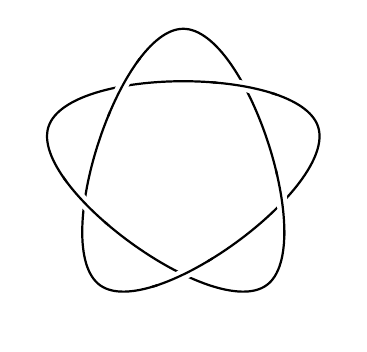
\begin{tikzpicture}[scale=0.9]
  % a pentagram with rounded tips: each piece runs from one tip to the next but one, 144° on
  \begin{knot}[consider self intersections, clip width=5, flip crossing/.list={2,4}]
    \strand[thick]
    (90:2) .. controls +(180:0.9) and +(144:0.9) .. (234:2) .. controls +(324:0.9) and +(288:0.9) .. (18:2) .. controls +(108:0.9) and +(72:0.9) .. (162:2)
      .. controls +(252:0.9) and +(216:0.9) .. (306:2) .. controls +(36:0.9) and +(0:0.9) .. cycle;
  \end{knot}
\end{tikzpicture}
